\section{Degree of Non-convexity}
TODO: intro
\begin{figure}
	\centering
	\begin{subfigure}[t]{1\columnwidth}
        		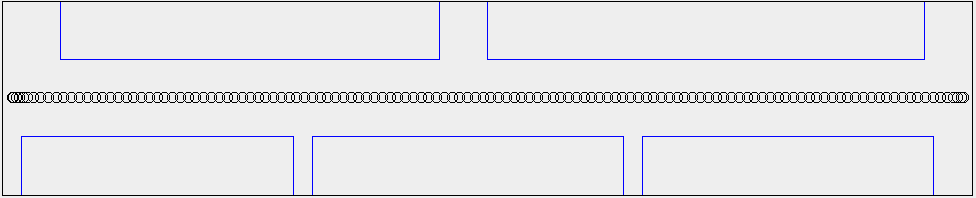
\includegraphics[width=\textwidth]{small-bench-flat}
        		\caption{The horizontal scenario.}
        		\label{fig:convex-straight}
	\end{subfigure}
	\par\bigskip
	\begin{subfigure}[t]{1\columnwidth}
        		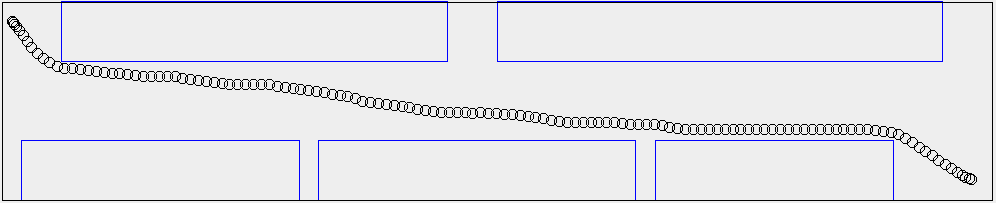
\includegraphics[width=\textwidth]{small-bench-diag}
        		\caption{The diagonal scenario.}
        		 \label{fig:convex-diag}
	\end{subfigure}	
	\par\bigskip
	\begin{subfigure}[t]{0.8\columnwidth}
        		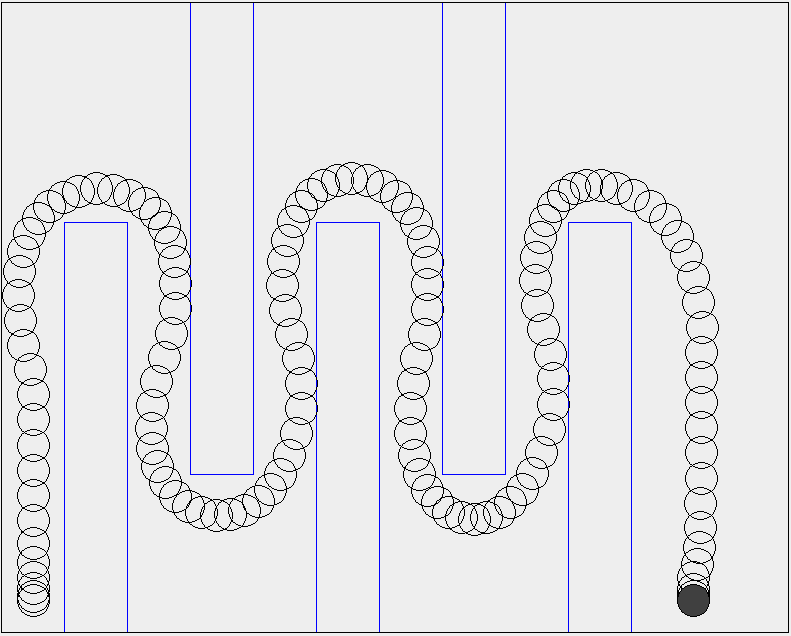
\includegraphics[width=\textwidth]{small-bench}
        		\caption{The Up/Down Scenario.}
        		 \label{fig:convex-full}
	\end{subfigure}	
    \caption{Three different testing scenarios, each with the same amount of obstacles. In each scenario, the UAV needs nearly the same amount of time steps to reach its goal. The only difference is the layout of the obstacles.}
    \label{fig:benchmarks}     
\end{figure}

\subsection{Scenarios}
\label{subsec:naive-scenarios}
\begin{figure}[]
	\centering
	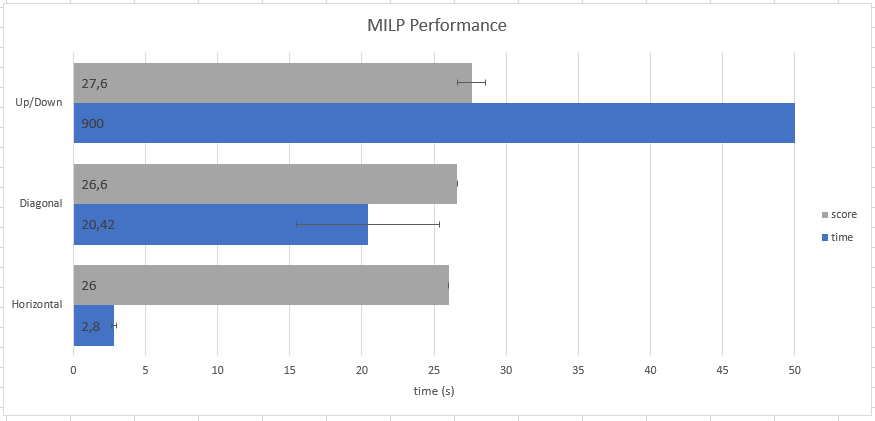
\includegraphics[width=\textwidth]{naive-performance}
	\caption{Performance of the MILP problem.}
	\label{fig:naive-performance}
\end{figure}
Typically, the amount of integer variables is used as a metric for the difficulty of a MILP problem. The amount of integer variables determines the worst case time needed to solve the MILP problem. An integer variable is needed for every edge, for every obstacle, for every time step. Increasing the amount of time steps and obstacles also increases the time needed to solve.\\
However, the amount of integer variables does not seem to be the only factor that determines the solve time. Figure \ref{fig:benchmarks} shows three different scenarios, each with the same amount of obstacles. The time step size is $0.2s$, and in each scenario there were 30 seconds worth of time steps. The scenarios are built such that the time needed for the UAV to reach the goal position is roughly the same (between 26 and 27 seconds). As a result, each scenario has the same amount of integer variables. With 4 edges for all 5 obstacles and 150 time steps, they each have 3000 integer variables to model the obstacles alone.\\

In the Horizontal scenario, the obstacles are not in the way of the UAV. The UAV can move in a straight line from the start position to its goal. In the Diagonal scenario, two of the obstacles are slightly in the way. The UAV is forced to make slight turns near the start and end of the trajectory. However, most of the trajectory is still straight. In the Up/Down scenario, the vehicle has to slalom around every obstacle.\\
\subsection{Results}
\label{subsec:naive-results}

Each scenario was solved five times. Figure \ref{fig:naive-performance} shows the time needed to solve the models, as well as the score. The score is also expressed in seconds, and is the time needed for the UAV to reach the goal position when following the generated trajectory. \\
The time needed to solve these scenarios varies dramatically. The Horizontal scenario is solved consistently in just under 3 seconds. The Diagonal scenario comes in at around 20 seconds, although the 95\% confidence interval is $\pm 4.9s$. The Up/Down scenario was limited to 900s of execution time. In this time, the solver could not find the optimal trajectory, which is why the score has a confidence interval.
\subsection{Discussion}
\label{subsec:naive-discussion}
Intuitively, it is not surprising that the Up/Down scenario is harder to solve than the other two. A human pilot would also have more difficulties navigating the Up/Down scenario compared to the others. However, this is cannot be determined by looking a the amount of integer variables or constraints alone.\\
Problems where the trajectory requires maneuvers seem to be harder to solve. The maneuvers are necessary because there are obstacles blocking a straight approach to the goal position. This observation led me to believe that the integer variables themselves do not cause the poor performance, but the real issue is what they model: a non-convex search space.\\
The amount of integer variables determines the worst-case performance because it determines the degree to which the search space can be non-convex. An informal definition of this degree of non-convexity would be the minimum amount of (possibly overlapping) convex shapes needed to reconstruct the original shape. With a single boolean variable, you need at most 2 convex shapes. With $n$ boolean variables, at most $2^n$ convex shapes are needed. TODO: cite.\\
\begin{figure}
	\centering
	\begin{subfigure}[t]{0.47\columnwidth}
        		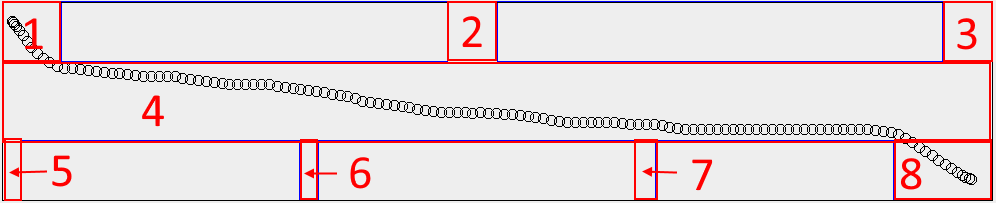
\includegraphics[width=\textwidth]{small-bench-diag-convexity}
        		\caption{8 convex regions are needed to reconstruct the diagonal scenario.}
        		 \label{fig:convex-diag-convexity}
	\end{subfigure}	
	\hfill
	\begin{subfigure}[t]{0.47\columnwidth}
        		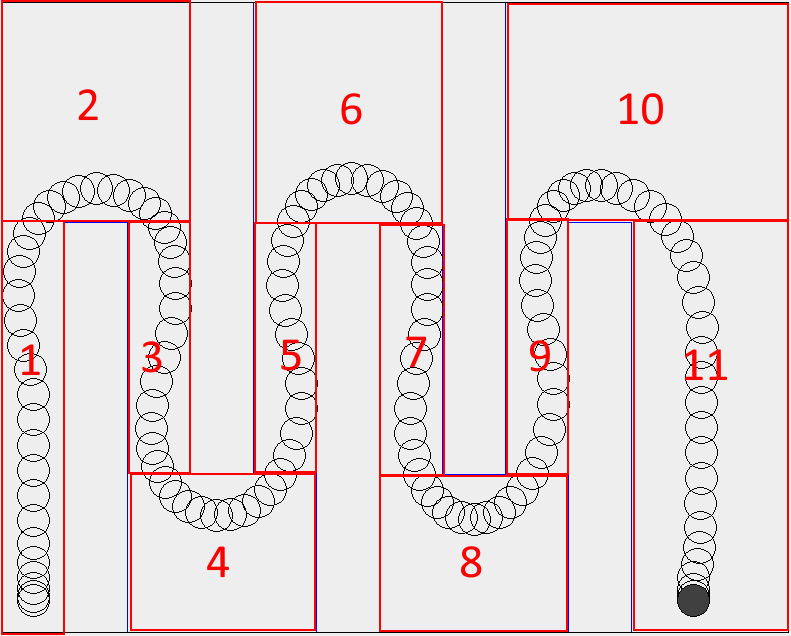
\includegraphics[width=\textwidth]{small-bench-convexity}
        		\caption{11 convex regions needed to reconstruct the Up/Down Scenario.}
        		 \label{fig:convex-full-convexity}
	\end{subfigure}	
    \caption{}
    \label{fig:benchmarks-convex}     
\end{figure}
The degree of convexity of the open space for the Up/Down scenario is 11 as shown in Figure \ref{fig:convex-full-convexity}. For the Horizontal and Diagonal scenarios, this is 8 as shown in Figure \ref{fig:convex-diag-convexity}. There is a difference, but this still does not seem like a good explanation. The Horizontal and Diagonal scenarios have the same degree of convexity, even though there's almost an order of magnitude difference in the solve times. \\
Even though the global degree of convexity is the same for the Horizontal and Diagonal scenarios, this is not the case for the neighborhood around the trajectory. In the Horizontal scenario, the trajectory only goes through a single convex region. In the Diagonal scenario, the trajectory goes through 3 convex regions. For the Up/Down scenario, the trajectory goes through all 11 regions. I present the following hypothesis:
\begin{hyp}
The degree of non-convexity around the optimal trajectory is a better indicator of the time needed to solve a MILP trajectory planning problem than the amount of integer variables.
\label{hyp:nonconvex}
\end{hyp}

%\subsection{Implications for the thesis}
%\label{subsec:naive-implications}
%While I present Hyptothesis \ref{hyp:nonconvex} before my algorithm, I actually only came up with it near the end of the project when the algorithm was already completed. The development of the algorithm was based on a lot of trial and error, exploiting the ideas that work and ignoring those that do not. MILP solvers are black boxes, so it is hard to predict which ideas will work and which do not. It is not uncommon for mathematically equivalent constraints to have drastically different effects on solve time. \\
%However, near the end of the project I started to understand the behavior of the solver better. Hypothesis \ref{hyp:nonconvex} is the result of what I have learned during the project. It is what I believe to be the core reason why my algorithm is effective.
%\par
%Section \ref{section:segment} often refers back to this hypothesis to motivate certain decisions. However, the hypothesis was often not the actual motivation behind those decisions. The arguments I present in section \ref{section:segment} are the arguments I believe to be correct at the time of writing.
%\par
%Due to time constraints, this thesis does not investigate Hypothesis \ref{hyp:nonconvex}. The outcome and conclusions of this thesis do not depend on this hypothesis


\section{Conclusions}
\label{section:conclusions}
Path planning using MIP was previously not computationally possible in large and complex environments. The approach presented in this paper shows that these limitations can effectively be circumvented by dividing the path into smaller segments using several steps of preprocessing. The specific algorithms used in each step to generate the segments can be swapped out easily with variations. Because the final path is generated by a solver, the constraints on the path can also be easily changed to account for different use cases. The experimental results show that the algorithm works well in realistic, city-scale scenarios, even when obstacles are distributed irregularly and dense.
\subsection{Future work}


%Another point that warrants attention are the transition between segments. In some cases, the UAV may end a segment in a state which causes issues in the next segment. This may cause the next segment to not be solvable, or result in a strange and undesirable trajectory. Overlapping the segments does help, but the algorithm can still not guarantee that the next segment will be feasible. Backtracking does guarantee that the next segment will be feasible, but at a great computational cost.\\
%This is partly due to active region generated by the genetic algorithm. Often the results are good, but in some cases the active region is very restrictive. The algorithm itself could certainly be improved, but it will be hard to guarantee a good result. Forcing the region to be significantly large solves the issue, but that comes at computational cost that may be too large.\\
%
%However, I do believe that these transition issues can be solved. One of the next extensions I would try is solving the MILP problem first with a higher time step size. Using this to roughly solve the current and next segment to provide a suitable goal state (including velocity) for the first segment would ensure a good start for the next segment as well. This may also allow for a lower approach margin multiplier, because the proper approach is already determined. \\
%


The obvious next step is extending this approach to 3D. The extra degree of freedom will likely come at a significant performance penalty, so this was not attempted during the thesis. One of the likely difficulties with the preprocessing as presented is that it treats all dimensions the same. This is fine for the horizontal dimensions, but due to gravity, movements the vertical dimension have different characteristics. The maximum acceleration of the UAV can no longer be assumed to be the same in all directions.\\
A possible mitigation to the increasing complexity of obstacles may be using a "2.5D" representation. A 2.5D obstacle is a 2D obstacle which also has a height value. This would only need one additional integer variable per obstacle to model. In a city scenario, this may be an acceptable approximation. \\

Another extension I would try is using moving to Mixed Integer Quadratic programming. Linear approximations to limit the length of vectors works, but it also introduces artifacts into the path. Increasing the amount of constraints that model the norm helps minimize the impact, but comes at a performance cost. Stating those constraints directly as a quadratic function would reduce the amount of constraints needed per time step. Even though the performance cost of a more accurate linear approximation is limited, this could still improve performance while increasing the accuracy of the model. Especially when the problem is also extended to 3D, since the this would require the linear approximation of a sphere instead of a circle. \\

\subsection{actual contribution}
\subsection{goals reached?}


\subsection{challenges}